\providecommand{\main}{..}
\documentclass[\main/main.tex]{subfiles}


\begin{document}


\section{Descriptive statistics}

\subsection{Sample size}
After the data cleaning, we are left with the following sample size (all waves together):

\begin{center}
    \begin{tabular}{llrr}

\toprule
{} & Country &     Male   &   Female     \\
\midrule
 & Austria &   5907 &   7871 \\
        & Belgium &   9415 &  11241 \\
        & Denmark &   6174 &   7060 \\
        & France &   7348 &   9414 \\
        & Germany &   6686 &   7494 \\
        & Italy &   8325 &   9807 \\
        & Spain &   8391 &  10130 \\
        & Sweden &   6625 &   7555 \\
        & Switzerland &   4437 &   5123 \\
\bottomrule
\end{tabular}
\end{center}

\subsection{Disability status}
Figure \ref{fig:disability_True} describes the distribution of disability status by gender and income decile. We consider the whole sample, i.e. individuals aged 50 years old or older, living in any of the nine selected countries and interviewed in any of the five waves. We notice that the majority of respondents reports being in a healthy status. However, there are some remarkable differences.




\begin{figure}[H]
    \centering
    \begin{minipage}{.5\textwidth}
        \centering
        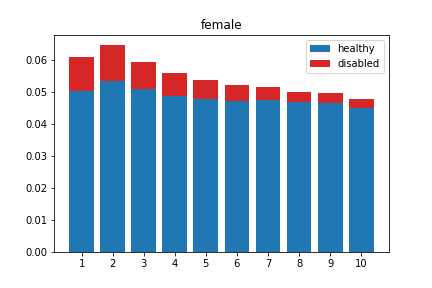
\includegraphics[scale=.5]{images/disability_female.png}
    \end{minipage}%
   \begin{minipage}{.5\textwidth}
        \centering
        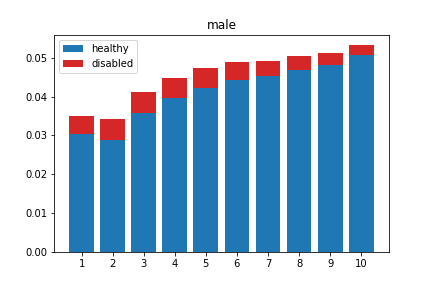
\includegraphics[scale=.5]{images/disability_male.png}
    \end{minipage}
    \caption{Percentage of individuals by gender, income, and disability status.}
    \label{fig:disability_True}
\end{figure}

\begin{figure}[H]
    \centering
    \begin{minipage}{.5\textwidth}
        \centering
        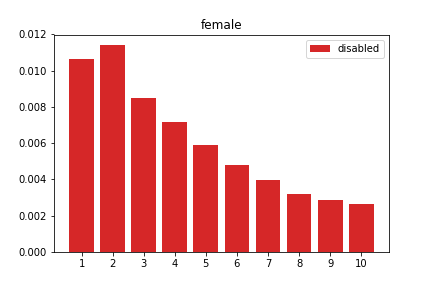
\includegraphics[scale=.5]{images/disability_only_female.png}
    \end{minipage}%
   \begin{minipage}{.5\textwidth}
        \centering
        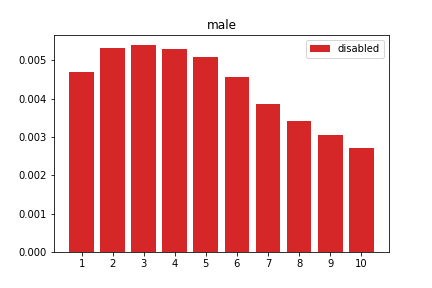
\includegraphics[scale=.5]{images/disability_only_male.png}
    \end{minipage}
    \caption{Percentage of disabled individuals by gender and income.}
    \label{fig:disability_True}
\end{figure}

First of all, income is not uniformly distributed across gender: there are more females in the lowest income percentiles than in the highest ones. For instance, around 6\% of the survey participants are female in the 1st income percentile as opposed to 5\% in the 10th income percentile. Conversely, men tend to have a higher income: 3.5\% of the participants are male in the 1st income percentile while 5.5\% are in the 10th income percentile. \\

Moreover, there appears to be a higher prevalence of disability status in the female population than in male one. For example, the peak of disability for female participants is around 1.2\% (in the 2nd income percentile), while for men it is around 0.55 \% (in the 3rd income percentile).\\

Finally, disability status appears to be decreasing with income, with respondents in the higher income percentiles being less likely to report a disability. However, these differences across groups appear more evident for females than for men, especially with respect to first 6 income percentiles.


\subsection{Age distribution}

To explore the data set more thoroughly, we plot the fitted distribution of the age variable for each income percentile and country. In figure \ref{fig:age_distr_germany} we present the plot that characterises the German sample. As we can see, younger people (i.e. between 50 and 70 years old) are more likely to belong to the highest income groups. This is an expected result as people in this age interval are likely to be working and earning a full salary, while older people are more likely to receive a pension income, which is typically lower.\\
However, the fact that the age distribution differs by income group should not bias our estimate, even though it might produce heterogeneity in the width of the confidence interval estimated for our prevalence data, i.e. the proportion of disabled to total population.




\begin{figure}[H]
        \centering
        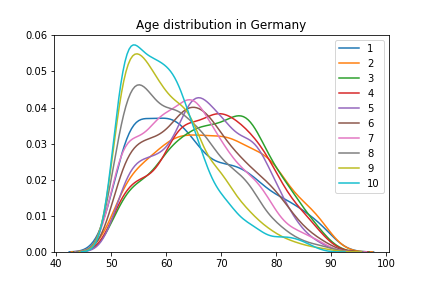
\includegraphics[scale=.5]{images/Age_distribution_in_Germany.png}
    \caption{Fitted distribution of age for the German sample.}
    \label{fig:age_distr_germany}
\end{figure}



\end{document}